\section{Probability Theory}\label{sec:probability-theory}


\indent
The central aim of modern probability theory is to provide a rigorous mathematical framework for modeling and analyzing phenomena involving uncertainty or randomness. This is achieved by building upon the foundations of measure theory, where probabilistic concepts are given precise measure-theoretic interpretations. The axiomatic framework, established by Andrey Kolmogorov, recasts probability in the language of measure spaces, where the "size" of a set of outcomes corresponds to its likelihood ~\cite[Chap 8]{MeasureTheoryLeGall}.

Just as measure theory confronts the impossibility of assigning a measure to all subsets of a general set (e.g., Vitali sets), probability theory restricts its focus to a collection of "events" that form a $\sigma$-algebra. An event is simply a set of possible outcomes to which a probability can be assigned. This structure ensures that logical combinations of events (e.g., "A or B", "A and B", "not A") are also events with well-defined probabilities.

\subsection{Probability Spaces}


\begin{definition}[Probability Space \textnormal{\cite{DurrettProbability}}]
    \label{def:probability-space}
    A \emph{probability space} is a measure space $(\Omega, \mathcal{F}, \mathbb{P})$ where:
    \begin{enumerate}[label=(\roman*)]
        \item $\Omega$ is a non-empty set, called the \emph{sample space}.
        \item $\mathcal{F}$ is a $\sigma$-algebra on $\Omega$. Its elements are called \emph{events}.
        \item $\mathbb{P}:\mathcal{F} \to [0, 1]$ is a \emph{probability measure} on $(\Omega, \mathcal{F})$, which is a measure satisfying the additional property that $\mathbb{P}(\Omega) = 1$.
    \end{enumerate}
\end{definition}

We will make a notational distinction between the general measure-theoretic framework and its probabilistic counterpart. In the former, we deal with a measure space $(X, \mathcal{A}, \mu)$, while in the latter, we work with a probability space $(\Omega, \mathcal{F}, \mathbb{P})$. The transition from measure theory to probability theory is straightforward: we simply impose the additional constraint that the total measure of the sample space $\Omega$ is $1$, thereby transforming our general measure into a probability measure. However, in probability theory, we are interested in mathematical model of random phenomena, where the sample space $\Omega$ represents all possible outcomes, and the $\sigma$-algebra $\mathcal{F}$ contains events of interest.


\begin{example}{\label{ex:probability-space}}
    It's worth noting some simple examples of probability spaces:
    \begin{itemize}
        \item \textbf{Rolling a die twice:} The sample space is $\Omega = \{1, 2, 3, 4, 5, 6\}^2$. Again, we take $\mathcal{F} = \mathcal{P}(\Omega)$. Then for any event $A \subseteq \Omega$, we define the probability measure $\mathbb{P}$ by
        \[
            \mathbb{P}(A) = \frac{|A|}{36},
        \]
        \item \textbf{Rolling a die until we get 6:} Here the sample space is not finite. It's possible that we roll the die 1000 times and not get a 6, even though the probability of this happening is very small. In this case, the sample space is
        \[
            \Omega = \{1, 2, 3, \dots, 6\}^{\mathbb{N}},
        \]
        while $\mathcal{F}$ is the smallest $\sigma$-algebra containing all sets of the form
        \[
            \{\omega \in \Omega \mid \omega_1 = i_1, \omega_2 = i_2, \dots, \omega_n = i_n\}\}
        \]
        where $n \in \mathbb{N}$ and $i_1, \dots, i_n \in \{1, \dots, 6\}$. Finally, the probability measure $\mathbb{P}$ such that for every choice of $n$ and $\omega_1, \dots, \omega_n$
        \[
            \mathbb{P}( \{\omega \in \Omega \mid \omega_1 = i_1, \omega_2 = i_2, \dots, \omega_n = i_n\}\}) = \frac{1}{6^n}.
        \]
        One can show that $P$ is unique such measure on $(\Omega, \mathcal{F})$ \cite[Chap 8]{MeasureTheoryLeGall}.
    \end{itemize}
\end{example}

In the general case of first example in~\ref{ex:probability-space}, if $\Omega$ is finite set and $\mathcal{F} = \mathcal{P}(\Omega)$, then the probability measure defined by
\[
    \mathbb{P}(\{\omega\}) = \frac{1}{|\Omega|} \quad \text{for all } \omega \in \Omega.
\]
We call this probability measure on $\Omega$ a \emph{uniform probability measure}. It assigns equal probability to each outcome in the sample space.

The properties of general measures translate directly into fundamental rules of probability.

\begin{lemma}
    Let $(\Omega, \mathcal{F}, \mathbb{P})$ be a probability space and let $A, B \in \mathcal{F}$.
    \begin{enumerate}
        \item $\mathbb{P}(A^c) = 1 - \mathbb{P}(A)$.
        \item If $A \subseteq B$, then $\mathbb{P}(A) \leq \mathbb{P}(B)$.
        \item $\mathbb{P}(A \cup B) = \mathbb{P}(A) + \mathbb{P}(B) - \mathbb{P}(A \cap B)$.
    \end{enumerate}
\end{lemma}

\begin{proof}

    These are direct consequences of the properties of a finite measure. For (1), since $A$ and $A^c$ are disjoint and their union is $\Omega$, we have $\mathbb{P}(A) + \mathbb{P}(A^c) = \mathbb{P}(A \cup A^c) = \mathbb{P}(\Omega) = 1$. The other properties follow from the lemmas in Section~\ref{sec:measure-theory}.
\end{proof}

\subsection{Random Variables}
In applications, we are often interested not in the outcomes themselves, but in some numerical quantity associated with them. This concept is formalized by a random variable, which is nothing more than a measurable function from the sample space to the real numbers.

\begin{definition}[Random Variable]
    \label{def:random-variable-prob}
    Let $(\Omega, \mathcal{F})$ be a measurable space and let $(\mathbb{R}, \mathcal{B}(\mathbb{R}))$ be the real line equipped with its Borel $\sigma$-algebra. A \emph{random variable} is a measurable function $X: \Omega \to \mathbb{R}$. That is, for every Borel set $B \in \mathcal{B}(\mathbb{R})$, the preimage is an event:
    \[
        X^{-1}(B) \coloneq \{\omega \in \Omega \mid X(\omega) \in B\} \in \mathcal{F}.
    \]
\end{definition}

This definition~\ref{def:random-variable-prob} is a direct specialization of a measurable function~\ref{def:measurable-function} to the context of probability. The measurability condition is crucial: it ensures that questions like "What is the probability that the random variable $X$ takes a value in the set $B$?" are well-posed, because the set of outcomes $\{\omega \mid X(\omega) \in B\}$ is guaranteed to be an event in $\mathcal{F}$ to which the measure $\mathbb{P}$ can be applied.

As with general measurable functions, we can use the proposition~\ref{prop:measurability-sufficient-cond} to simplify the verification that a function is a random variable. Since the collection of intervals $\mathcal{C} = \{(-\infty, x] \mid x \in \mathbb{R}\}$ generates the Borel $\sigma$-algebra $\mathcal{B}(\mathbb{R})$, a function $X: \Omega \to \mathbb{R}$ is a random variable if and only if $\{\omega \in \Omega \mid X(\omega) \leq x\} \in \mathcal{F}$ for all $x \in \mathbb{R}$.

Note that, the topology on $\mathbb{R}$ is generated by the open intervals, hence the Borel $\sigma$-algebra $\mathcal{B}(\mathbb{R})$ is generated by the collection of open intervals in $\mathbb{R}$. Therefore, a random variable $X$ is $\mathcal{F}$-measurable if and only if for every open interval $(a, b)$, the preimage $X^{-1}((a, b))$ is in $\mathcal{F}$.

Recall, the indicator function defined in~\ref{eq:indicator-function-def}, which can be

\begin{example}[Indicator functions]
    \label{ex:indicator-function-in-probability}
    Let $(\Omega, \mathcal{F}, \mathbb{P})$ be a probability space and consider the indicator function for any set $A \in \mathcal{F}$
    \[
        \begin{aligned}
            \mathds{1}_A: \Omega &\to \{0, 1\} \subseteq \mathbb{R} \\
            \omega &\mapsto \begin{cases}
                               1 & \text{if } \omega \in A \\
                               0 & \text{if } \omega \notin A.
            \end{cases}
        \end{aligned}
    \]
    It follows from this definition that $\mathds{1}_A$ is measurable for any $A \in \mathcal{F}$, hence it's a random variable.
\end{example}

\begin{example}{\label{ex:random-variable}}
    We are going back to the examples we considered in the previous section~\ref{ex:probability-space}.
    \begin{itemize}
        \item \textbf{Rolling a die twice:} Let $X: \Omega \to \mathbb{R}$ be defined by
        \[
            X(\omega) = \omega_1 + \omega_2 \in \{2, 3, \dots, 12\}
        \]
        where $\omega = (\omega_1, \omega_2) \in \Omega$.
        Then for any $x \in \{2, 3, \dots, 12\}$, the event $\{\omega \in \Omega \mid X(\omega) = x\}$ is measurable, since it can be expressed as a finite union of sets of the form $\{\omega \in \Omega \mid \omega_1 = i_1, \omega_2 = i_2\}$. For example,
        \[
            \begin{aligned}
                X^{-1}([2, 4]) &= \{\omega \in \Omega \mid 2 \leq X(\omega) \leq 4\} \\
                &= \{\omega \in \Omega \mid (\omega_1, \omega_2) \in \{(1, 1), (1, 2), (2, 1), (1, 3), (2, 2), (3, 1)\}\}.
            \end{aligned}
        \]
        So, $X^{-1}([2, 4]) \in \mathcal{F} = \mathcal{P}(\Omega)$.
        \item \textbf{Rolling a die until we get 6:} Let $X: \Omega \to \mathbb{R}$ be defined by
        \[
            X(\omega) = \inf\{j: \omega_j = 6\}
        \]
        with the convention that $\inf{\emptyset} = \infty$. In this case $X^{-1}([2, 4])$ is union given below:
        \[
            \begin{aligned}
                X^{-1}([2, 4]) = \{&\omega \in \Omega \mid \omega_1 \neq 6, \omega_2 = 6\} \\
                &\cup \{\omega \in \Omega \mid \omega_1 \neq 6, \omega_2 \neq 6, \omega_3 = 6\} \\
                &\cup \{\omega \in \Omega \mid \omega_1 \neq 6, \omega_2 \neq 6, \omega_3 \neq 6, \omega_4 = 6\}.

            \end{aligned}
        \]
    \end{itemize}
\end{example}

\subsection{Distributions of random variables}

A random variable $X$ on a probability space $(\Omega, \mathcal{F}, \mathbb{P})$ induces a new probability measure on its codomain $(\mathbb{R}, \mathcal{B}(\mathbb{R}))$. This induced measure is called the \emph{distribution} or \emph{law} of the random variable.

\begin{definition}[Distribution of a Random Variable]
    Let $X$ be a random variable on $(\Omega, \mathcal{F}, \mathbb{P})$. The \emph{(probability) distribution} of $X$ is the probability measure $P_X:\mathcal{B}(\mathbb{R}) \to [0, 1]$ on $(\mathbb{R}, \mathcal{B}(\mathbb{R}))$ defined by
    \[
        P_X(B) \coloneq \mathbb{P}(X^{-1}(B)) \quad \text{for all } B \in \mathcal{B}(\mathbb{R}).
    \]
    This is also known as the \emph{pushforward measure} of $\mathbb{P}$ by $X$.
\end{definition}

The distribution $P_X$ captures all the probabilistic information about $X$ without reference to the original sample space $\Omega$. A closely related concept is the cumulative distribution function (CDF), which is simply a probability measure on the real line that describes the likelihood of $X$ taking values less than or equal to a given threshold.

\begin{definition}[Cumulative Distribution Function (CDF)]
    \label{def:cdf}
    The \emph{CDF} of a random variable $X$ is the function $F_X: \mathbb{R} \to [0, 1]$ defined by
    \[
        F_X(x) \coloneq \mathbb{P}(\{\omega \in \Omega \mid X(\omega) \leq x\}) = \mathbb{P}(X \leq x).
    \]
    In terms of the distribution, $F_X(x) = P_X((-\infty, x])$.
\end{definition}

\begin{remarknl}
    Note that, CDF $F_X$ in~\ref{def:cdf} uniquely determines the probability measure $P_X$~\cite[Thm 12.4]{ProbabilityBillingsley}. Moreover, by~\cite[Sec. 14.4]{ProbabilityBillingsley}
    \[
        \lim_{x \to -\infty}F_X(x) = 0 \text{ and } \lim_{x \to \infty}F_X(x) = 1.
    \]
\end{remarknl}

\begin{example}
    We illustrate these definitions by going back to our running examples.
    \begin{itemize}
        \item \textbf{Rolling a die twice:} Recall, $X^{-1}([2, 4])$ from previous example~\ref{ex:random-variable}. Then
        \[
            P_X([2, 4]) = \mathbb{P}(X^{-1}([2, 4])) = \mathbb{P}(\{\omega \in \Omega \mid X(\omega) \in [2, 4]\}) = \frac{6}{36} = \frac{1}{6}.
        \]
        Meanwhile, the CDF is given by
        \[
            F_X(4) = \mathbb{P}(X \leq 4) = \mathbb{P}(\{\omega \in \Omega \mid X(\omega) \leq 4\}) = \frac{1}{6}
        \]
        In this case, $P_X([2, 4]) = F_X(4)$ since $X^{-1}(\{1\}) = \emptyset$ (the event that the sum of two dice is less than 2 is impossible). However, one can show that $P_X([3, 5]) = F_X(5) - F_X(2)$.
        \begin{figure}[h]
            \centering
            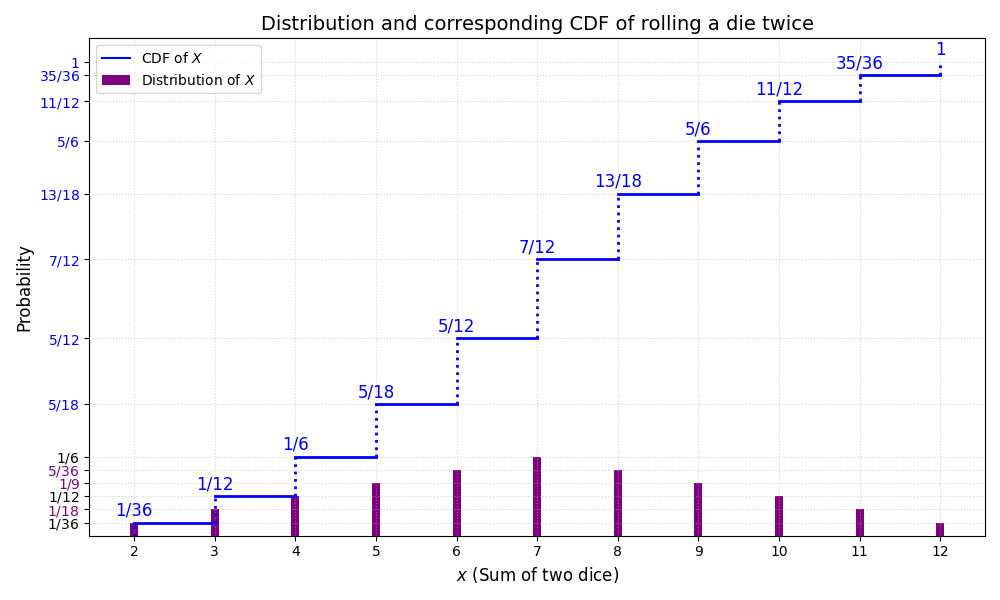
\includegraphics[scale=0.45]{chapter-1/sections/img}
            \caption{Two different characteristics of the random variable $X$ defined by the sum of two dice.\label{fig:figure-distribution-random-variable}}
        \end{figure}
        \item \textbf{Rolling a die until we get 6:} In this case, the random variable $X$ takes values in $\mathbb{N} \cup \{\infty\}$. The distribution of $X$ is given by
        \[
            P_X(\{n\})  = \mathbb{P}(\{\omega \in \Omega \mid X(\omega) = n\}) = \frac{5^{n-1}}{6^n} \quad \text{for } n \in \mathbb{N},
        \]
        However, in this case $F_X$ is
        \[
            \begin{aligned}
                F_X(n) &= P(\{\omega \in \Omega \mid  X(w) \leq n \}) \\
                &= P_X(\{1, \dots, n\}) \\
                &= \sum_{k=1}^n P_X(\{k\}) \\
                &= \sum_{k=1}^n \frac{5^{k-1}}{6^k} = 1 - \frac{5^n}{6^n}.
            \end{aligned}
        \]
        The visualisation of distribution and CDF of this random variable is shown in Figure~\ref{fig:figure-distribution-random-variable-2}.
        \begin{figure}[h]
            \centering
            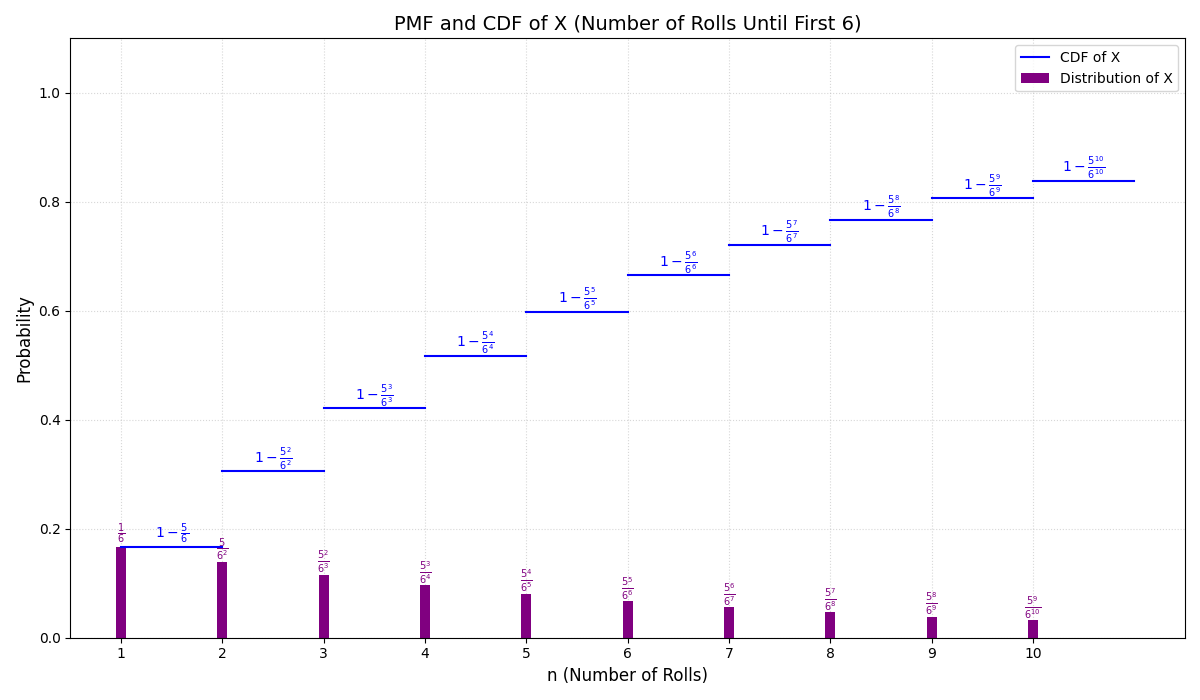
\includegraphics[scale=0.35]{chapter-1/sections/img_1}
            \caption{Two different characteristics of the random variable $X$ defined by the amount of rolls until we get $6$.\label{fig:figure-distribution-random-variable-2}}
        \end{figure}
    \end{itemize}
\end{example}

Certain distributions appear so frequently in theory and applications that they are given special names. These distributions can be \emph{discrete}, where the random variable takes values in a countable set, or \emph{continuous}.

\begin{example}[Classical Distributions]
    \label{ex:classical-distributions}
    Below are two foundational examples of discrete distributions.

    \begin{itemize}
        \item \textbf{The Uniform Distribution.} Let $(\Omega, \mathcal{F}, \mathbb{P})$ be a probability space and  $X: \Omega \to \mathbb{R}$ be a random variable that takes finitely many distinct values, say $\{a_1, \dots, a_n\} \subseteq \mathbb{R}$. We say $X$ has a uniform distribution if each outcome is equally likely. The probability is given by:
        \[
            P_X(\{a_i\}) = \frac{1}{n}, \quad \forall a_i \in \{a_1, \dots, a_n\} \subseteq \mathbb{R}.
        \]
        A random variable that returns the value on upper face of a fair six-sided die roll is an example of uniformly distributed random variable where $X(\omega) \in \{1, 2, 3, 4, 5, 6\}$ and each outcome is equally likely.

        \item \textbf{The Bernoulli Distribution.} This is the distribution of a random variable $X$ with values in $\{0, 1\}$, governed by a parameter $p \in [0, 1]$:
        \[
            P_X(\{1\}) = p \quad \text{and} \quad P_X(\{0\}) = 1 - p.
        \]
        This distribution models a single trial with two possible outcomes, often interpreted as "success" (1) and "failure" (0), such as a single toss of a potentially biased coin.
    \end{itemize}
\end{example}

It is worth noting that these definitions can overlap. A random variable representing a single fair coin toss (e.g., mapping heads to 1 and tails to 0) follows a Bernoulli distribution with parameter $p=1/2$. At the same time, it also follows the uniform distribution on the finite set $E=\{0, 1\}$, since each outcome has probability $1/|E| = 1/2$.

\subsection{Expected value of a random variable}

The final core concept is the expectation, which formalizes the intuitive idea of the 'average' or 'mean' value of a random variable. For a variable that takes on a finite set of values, its expectation is computed as a weighted average, with the probabilities serving as weights. When a random variable takes on a continuous range of values, this weighted average is calculated via integration. In the definition below, we denote the absolute value of a random variable $X$ by $|X|$.

\begin{definition}[Expected Value]
    Let $X$ be a random variable on a probability space $(\Omega, \mathcal{F}, \mathbb{P})$. The \emph{expected value} (or \emph{expectation}) of $X$, denoted $E[X]$, is its integral with respect to the probability measure $P$:
    \[
        E[X] \coloneq \int_{\Omega} X(\omega) \, d\mathbb{P}(\omega).
    \]
    The expectation is said to exist if this integral is well-defined (specifically, if $E[|X|] < \infty$).
\end{definition}

The well-definedness condition of the expectation integral is crucial and is discussed in detail in \cite[Chap 8]{MeasureTheoryLeGall}. It's outside the scope of this dissertation to delve into the intricacies of this condition, but we will provide a brief overview of how the expectation is constructed for random variables.

\begin{example}
    Following the setup in~\ref{ex:indicator-function-in-probability}, consider the indicator function $\mathds{1}_A: \Omega \to \mathbb{R}$ for an event $A$. The expectation of an indicator function is simply the probability of the event it represents:
    \[
        E[\mathds{1}_A] = \mathbb{P}(A) \times 1 + \mathbb{P}(X \setminus A) \times 0 = \mathbb{P}(A).
    \]
\end{example}

From these, we can construct random variables that take a finite number of values.

\begin{definition}[Simple Random Variable]
    Let $(\Sigma, \mathcal{F}, P)$ be a probability space. A random variable $X: \Sigma \to \mathbb{R}$ is called a \emph{simple random variable} if it can be written as a finite linear combination of indicator functions:
    \[
        X = \sum_{i=1}^n a_i \mathds{1}_{A_i},
    \]
    where $a_i \in \mathbb{R}$ are the distinct values taken by $X$ and $A_i = X^{-1}(\{a_i\})$ are the corresponding disjoint events.
\end{definition}

It's important to note that if $X$ is such simple random variable taking finitely many values $\{a_1, \dots, a_n\} \subseteq \mathbb{R}$, then
\[
    \begin{aligned}
        \Omega &= X^{-1}(\{a_1\}) \cup X^{-1}(\{a_2\}) \cup \dots \cup X^{-1}(\{a_n\}) \\
        &= A_1 \cup A_2 \cup \dots \cup A_n,
    \end{aligned}
\]
Hence, we can use the linearity of $X$ to compute the expectation of a simple random variable:
\[
    E[X] = \sum_{i=1}^n a_i E[\mathds{1}_{A_i}] = \sum_{i=1}^n a_i \mathbb{P}(A_i).
\]

%The formal construction of the expectation integral then proceeds as follows:
%\begin{enumerate}
%    \item For a \textbf{simple random variable} $X = \sum_{i=1}^n a_i \mathbf{1}_{A_i}$, the expectation is defined as the weighted average:
%    \[
%        E[X] = \sum_{i=1}^n a_i P(A_i).
%    \]
%    \item For a \textbf{non-negative random variable} ($X \geq 0$), the expectation is defined by approximating $X$ from below with simple random variables:
%    \[
%        E[X] = \sup \{ E[Y] \mid Y \text{ is simple and } 0 \leq Y \leq X \}.
%    \]
%    \item For a \textbf{general random variable}, we decompose it into its positive and negative parts, $X = X^+ - X^-$, where $X^+ = \max(X, 0)$ and $X^- = \max(-X, 0)$. The expectation is then:
%    \[
%        E[X] = E[X^+] - E[X^-],
%    \]
%    provided that at least one of the terms on the right is finite.
%\end{enumerate}

\begin{example}
    Let's apply this definition to our running examples.
    \begin{itemize}
        \item \textbf{Rolling a die twice:} The random variable $X$, representing the sum of the outcomes, is a simple random variable taking values in $\{2, 3, \dots, 12\}$. We can directly apply the formula from step 1:
        \[
            E[X] = \sum_{k=2}^{12} k \cdot P_X(\{k\}).
        \]
        Calculating the probabilities for each sum (e.g., $\mathbb{P}(\{2\})=1/36$, $\mathbb{P}(\{3\})=2/36$, etc.), we find:
        \[
            \begin{aligned}
                E[X] &= 2 \cdot P_X(\{2\}) + 3 \cdot P_X(\{3\}) + \dots + 12 \cdot P_X(\{12\}) \\
                &= 2 \cdot \frac{1}{36} + 3 \cdot \frac{2}{36} + \dots + 12 \cdot \frac{1}{36} = 7\\
            \end{aligned}
        \]
        \item \textbf{Rolling a die until we get 6:} The random variable $X$, representing the number of rolls, is a non-negative but not simple random variable. Its expectation is found using the definition for non-negative variables, which for a discrete variable taking values in $\mathbb{N}$ simplifies to the infinite sum:
        \[
            \begin{aligned}
                E[X] &= \sum_{n=1}^{\infty} n \cdot P_X(\{n\}) \\
                &= \sum_{n=1}^{\infty} n \cdot \frac{5^{n-1}}{6^n} = \frac{1}{6} \sum_{n=1}^{\infty} n \left(\frac{5}{6}\right)^{n-1} \\
                &= \frac{1}{6} \cdot \frac{1}{(1 - 5/6)^2} = \frac{1}{6} \cdot 36
            \end{aligned}
        \]
        This means we expect to wait 6 rolls on average to see the first 6.
    \end{itemize}
\end{example}

%\begin{example}[Continuous Random Variable]
%    When a random variable's distribution is described by a \emph{probability density function} (pdf) $f_X(x)$, the abstract expectation integral simplifies to a more familiar Riemann-style integral. For a random variable $X$ following the Uniform distribution on $[0, 1]$, the pdf is $f_X(x) = 1$ for $x \in [0, 1]$ and 0 otherwise. The expectation is:
%    \[
%        E[X] = \int_{-\infty}^{\infty} x f_X(x) \, dx = \int_0^1 x \cdot 1 \, dx = \left[ \frac{x^2}{2} \right]_0^1 = \frac{1}{2}.
%    \]
%    This confirms the intuition that the average value of a number chosen uniformly from the interval $[0, 1]$ is its midpoint.
%\end{example}